\documentclass[12pt, letterpaper]{article}
\usepackage[utf8]{inputenc}
\usepackage{graphicx}
\usepackage{hyperref}
\usepackage{fancyvrb}
\usepackage{array}
\usepackage{biblatex}
\usepackage{float}
\bibliography{rapport} 

\title{Fiche de lecture : Réseau neuronal convolutif}
\author{Chaolei Cai
\\
    \multicolumn{1}{
        p{.7\textwidth}}{\centering\emph{Université Paris Vincennes St-Denis\\
  UFR mathématiques, informatique, technologies sciences de l'information\\}
  L3 Informatique}
}
\date{\today}
\begin{document}


\begin{titlepage}
    \maketitle
\end{titlepage}

\tableofcontents

\section{Avant-propos}
Ce document est ma fiche de lecture sur le réseau neuronal convolutif (Convolutional Neural Network or ConvNet), il fait partie de la notation pour 
le cours de programmation pour l'intelligence artificiel enseigné par M.Jean-Jacques Mariage aux L3 de la licence informatique.\\
Dans le plan géneral, je vais vous présenter le néocognitron, un ancêtre des CNN.\\
Dans un second temps, je vais m'intéresser à une publication d'Alex \\Krizhevsky, Ilya Sutskever et Geoffrey E.Hinton sur la classfication d'image via un Deep Convolutional Neural Networks.\\
Puis je reviendrai à des sujets plus récente "Batch normalization" proposé par Sergey Ioffe et Christian Szegedy, il s'agit de la méthode de regularization la plus moderne sur les CNN.
Enfin je terminerai sur un article de Amir Rosenfeld, Richard Zemel et John K. Tsotsos qui pointe les limites rencontrées par les modèles CNN les plus moderne.

\section{Néocognitron}
\subsection{Présentation de l'auteur : Kunihiko Fukushima}
M.Fukushima est un chercheur en informatique connue pour ses travaux dans le domaine du réseau de neuronne artificiel et du deep learning.
Le plus célèbre étant son modèle de Néocognitron publié en 1980 \autocite{Fukushima:1}.

\subsection{Présentation de l'article}
Le néocognitron est un modèle élaboré depuis le modèle de cognitron publié par le même auteur en 1975. 
Il s'agit d'un réseau de neuronne multi-couche auto-organisatrice. L'apprentissage n'est pas supervisée, c'est à dire que 
les données ne sont pas étiquetées. Il s'inspire notamment des travaux de Hubel et Wiesel sur le système visuel animal (chat). A nos jour, la recherche a bien évidemment avancé depuis 1959, Le model d'Hubel et Wiesel n'est plus tout à fait exacte 
mais reste intéressant dans les grandes lignes. Un des professeur en physiologie m'avait d'ailleurs présenté ces travaux quand j'étudiais encore à la 
licence Science pour la santé à Paris Descartes quelques années auparavant. \\
Le point important à retenir c'est que Hubel et Wiesel propose l'idée qu'un reseau de neuronne est 
constitué de cellule "Simple" appelée "S-cells" et de cellule "Complex" appelée "C-cells".\\
Pour être tout à fait précis, le neocognitron ne reconnais pas l'object complexe mais présente plutôt un 
capacité à reconnaitre des patternes de stimuli précis après l'entraînement.\\
Notre sujet présente une organisation étalé sur plusieurs couche, dans l'idée, il faut retenir qu'il s'agit d'un reseau organisé en cascade et hierarchisé.

\subsection{Présentation de la structure}
Au niveau de l'entrée, nous pouvons trouver des cellules photoreceptrices chargées de transmettre l'information. Si nous devons faire un rapprochement avec le réel, cela correspond aux rétines sensible à différentes stimulis lumineuse.\\
Dans la suite intervient une succession de module, une module est constitué d'une ou plusieurs couche de neuronnes.
La première constituée de cellules simples, l'auteur appelle cette couche "S-layer", puis arrive les couches complexes constituées 
à leur tour de cellules complexe voire hyper-complexe, de la même manière, ils portent le nom de "C-layer".
Il est intéressant de noter que seul les synapses partant vers une "S-cell" ont la propriété de plasticité. La plasticité en neuroscience 
est le terme pour désigner le capacité d'un neuronne à former et modifier ses connexions vers d'autre neuronne via les synapses. 



\begin{figure}[H]
    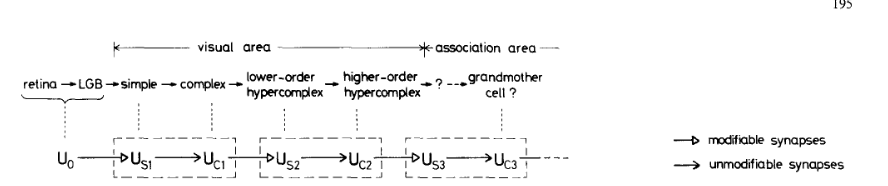
\includegraphics[width=\linewidth]{img/fig1.png}
    \caption{Correspondence between the hierarchy model by Hubel and Wiesel, and the neural network of the neocognitron}
    \label{fig:L1}
\end{figure}

Comme vous pouvez le voir sur ce schéma, U0 est notre couche d'entrée, par la suite intervient une cascade de module constitué par différentes couches de cellules.
Au sein d'une même module, les liens entre les neuronnes de différentes couches sont fixes, alors qu'à la jointure des 
modules, ces liens sont modifiables et peuvent être amènés à évoluer au fur et à mesure de l'apprentissage.
Tout cela nous permet de faire un parallèle avec le fonctionnement du cortex visuel et associatif. 
\newpage
\printbibliography
\end{document}
